\section{The Mechanical System}

\subsection{Preface to the Section}
Most of the mechanical components on board the vehicle were installed by the SCOPE team that first worked on the vehicle in 2009 - 2010. As such, many parts of this section will begin with pages from the original SCOPE reports and then followed by supplementary information on what might have changed since the SCOPE report was written. 
%
Today, this mechanical system remains largely the same except for the following changes:

\subsection{The Electronics Box}

The electronics box mounted to the back of the vehicle is, of course, where most of the electronics including the computers, FPGA chassis, the power supplies, and most of the power distribution elements on the vehicle are housed.\\ \\
%
\noindent The electronics box is essentially a heavily modified Nothern Tools Co. metal tool box that is mounted on two vibration isolating rails in the bed of the vehicle. This mounting system consists of two pieces of square channel high tensile strength steel with corrosion resistant coating that is bolted to the bed of the vehicle. The box is then attached to the steel with four vibration-damping sandwich mounts allowing for a relatively smooth ride. This simple system is robust and requires relatively little assembly. The vehicle also includes a roof-mounted optics-quality pegboard for sensor mounting. 

\begin{enumerate}
\item The monitor mentioned in the original SCOPE team report is the Nortec SUN-1710-P daylight-visible monitor. The current monitor on the vehicle is a standard Acer monitor
\end{enumerate}

\newpage

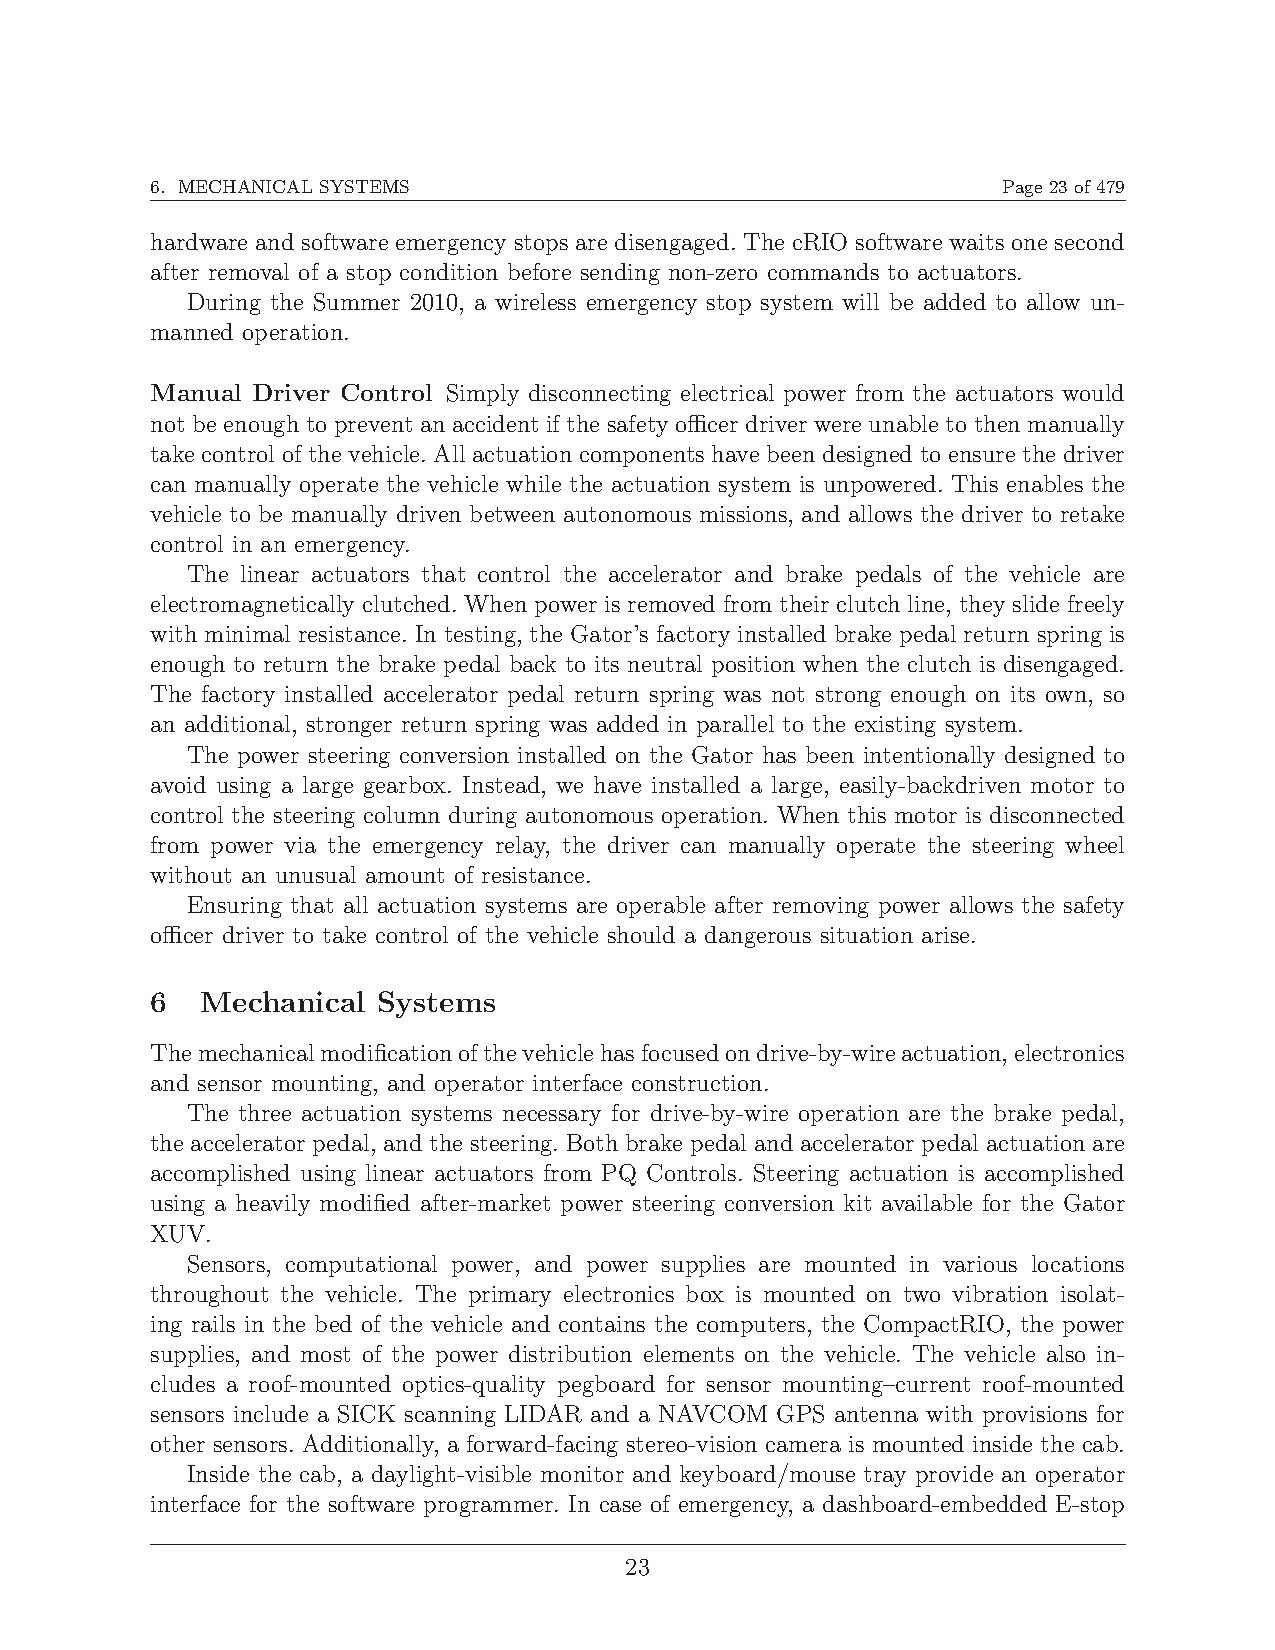
\includepdf[scale=0.9, pages=-, clip, trim=0mm 20mm 0mm 35mm, pagecommand={}]{MechSystem.pdf}

\newpage

\subsection{Additional Mechanical Components}